\section{Participant 5}

%HS

\subsection{Date \& Time}
\begin{table}[ht]
  \begin{tabular}{|P{3cm}|P{3cm}|}
	\multicolumn{2}{c}{\textbf{2016-08-09}}    	\\ \hline
    Start Time      			& End Time   					\\ \hline
   \textbf{15:49:28} 	& \textbf{17:20:58}    	\\ \hline
   \multicolumn{2}{c}{Duration}    						\\ \hline
   \multicolumn{2}{c}{\textbf{01:31:30}} 			\\ \hline
  \end{tabular}
  \newline\newline
  \caption{P5: Date and Time}\label{dandt5}
\end{table}

\FloatBarrier

\subsection{Questions}
\begin{itemize} 
  \item[\Checkmark] Are you a Student?
  \item[\XSolidBrush] Did you work in a team?
  \item[\XSolidBrush] Did you listen to music?
  \item[\XSolidBrush] Did you feel tired?
  \item[\Checkmark] Did you enjoy the tasks?
  \item[\Checkmark] Did you give all you attention to the tasks?
  \item[\XSolidBrush] Were you distracted during the tasks?
  \item[\XSolidBrush] Did you feel stressed
  \item[\XSolidBrush] Do you think the tasks were easy?  
\end{itemize}


\FloatBarrier
\newpage
\subsection{Accelerometer}

\begin{figure}[ht]
	\centering
	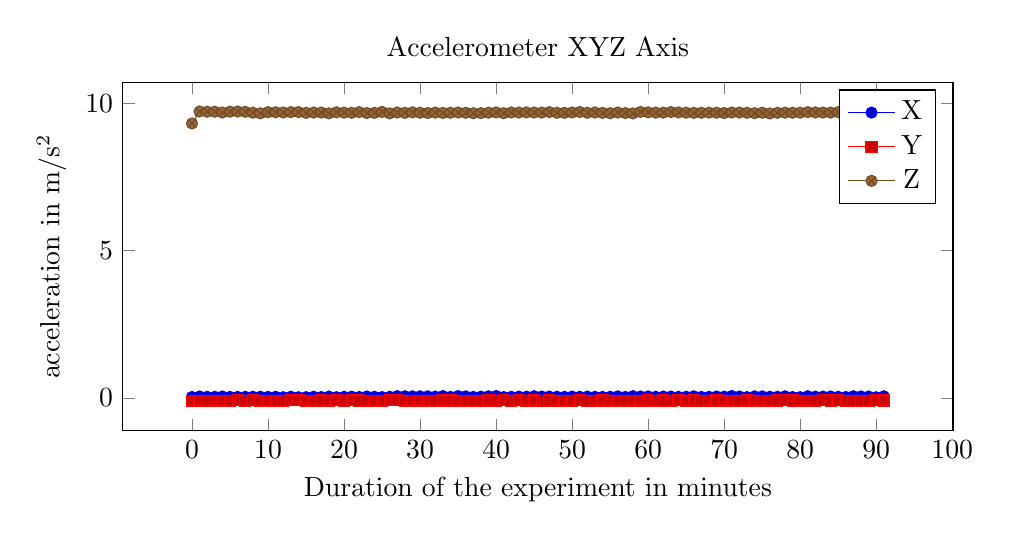
\begin{tikzpicture}
\begin{axis}[
	height=6cm,
	width=\textwidth,
	xlabel=Duration of the experiment in minutes,
	ylabel=acceleration in m/s$^2$,
	title=Accelerometer XYZ Axis,
	unbounded coords=discard],
	
%X
\addplot coordinates {
(0 , 0.028624852325)
(1 , 0.0456503159435)
(2 , 0.0345175602857)
(3 , 0.0348083495)
(4 , 0.04493713425)
(5 , 0.03185272225)
(6 , 0.032054901)
(7 , 0.0333658853333)
(8 , 0.03527832025)
(9 , 0.037109375)
(10 , 0.0322875975)
(11 , 0.036422729)
(12 , 0.02068481454)
(13 , 0.0372229681111)
(14 , 0.0187072753833)
(15 , 0.02278137175)
(16 , 0.0373102818333)
(17 , 0.0263108474615)
(18 , 0.0425605775)
(19 , 0.021026611)
(20 , 0.0350392652833)
(21 , 0.0383300785)
(22 , 0.0275421141)
(23 , 0.0451100666667)
(24 , 0.035198212)
(25 , 0.023899078475)
(26 , 0.035690308)
(27 , 0.05596923825)
(28 , 0.05286331185)
(29 , 0.0494931539167)
(30 , 0.0507286924444)
(31 , 0.0508575438)
(32 , 0.0422706605)
(33 , 0.0589447026667)
(34 , 0.03134918226)
(35 , 0.0602783198)
(36 , 0.0494422905)
(37 , 0.031689962)
(38 , 0.039909362)
(39 , 0.050775147)
(40 , 0.0615295414)
(41 , 0.0245971678667)
(42 , 0.0336181642)
(43 , 0.04070663425)
(44 , 0.038182577)
(45 , 0.05458831725)
(46 , 0.043797811)
(47 , 0.0426910398)
(48 , 0.0372436522)
(49 , 0.0326446532)
(50 , 0.0426849356)
(51 , 0.0350494386667)
(52 , 0.04183197075)
(53 , 0.03400802625)
(54 , 0.030904134)
(55 , 0.034921264)
(56 , 0.049016317)
(57 , 0.0298919676667)
(58 , 0.055935669)
(59 , 0.045284271)
(60 , 0.0474853525)
(61 , 0.0355326333333)
(62 , 0.04415130625)
(63 , 0.04241180425)
(64 , 0.0335184733333)
(65 , 0.0360717774)
(66 , 0.05042648375)
(67 , 0.03061294525)
(68 , 0.0333030008182)
(69 , 0.0442055152105)
(70 , 0.040286255)
(71 , 0.0616607675)
(72 , 0.0454444895)
(73 , 0.024180095)
(74 , 0.049064636)
(75 , 0.0488922114)
(76 , 0.03613281275)
(77 , 0.03391647325)
(78 , 0.0513407386667)
(79 , 0.0258255005)
(80 , 0.023609161425)
(81 , 0.054763794)
(82 , 0.0396626796667)
(83 , 0.04229354875)
(84 , 0.0447021485)
(85 , 0.0336486822)
(86 , 0.0279922485)
(87 , 0.0545578005)
(88 , 0.0470581055)
(89 , 0.0445327755)
(90 , 0.019207001)
(91 , 0.05170059225)
};

%Y
\addplot coordinates {
(0 , -0.09772237125)
(1 , -0.108810424783)
(2 , -0.103489468571)
(3 , -0.105393982)
(4 , -0.1029891965)
(5 , -0.09886169375)
(6 , -0.087383271)
(7 , -0.0943857833333)
(8 , -0.08496475)
(9 , -0.0982716866667)
(10 , -0.09655761625)
(11 , -0.0961120602)
(12 , -0.107305908)
(13 , -0.081837973)
(14 , -0.0802561431667)
(15 , -0.095504761)
(16 , -0.0975189198333)
(17 , -0.0929166354615)
(18 , -0.097572326)
(19 , -0.0717506415)
(20 , -0.0957183841667)
(21 , -0.08687210025)
(22 , -0.09144973825)
(23 , -0.09747823)
(24 , -0.101642611)
(25 , -0.1035652175)
(26 , -0.066518148)
(27 , -0.08568573)
(28 , -0.10135345475)
(29 , -0.102905273208)
(30 , -0.10242886)
(31 , -0.1043487568)
(32 , -0.102169036)
(33 , -0.091405232)
(34 , -0.09143066375)
(35 , -0.1044128416)
(36 , -0.10267639)
(37 , -0.1101964315)
(38 , -0.1020584125)
(39 , -0.0895660396)
(40 , -0.1017395028)
(41 , -0.0832926433333)
(42 , -0.102542115)
(43 , -0.087623596)
(44 , -0.0957692433333)
(45 , -0.09049987875)
(46 , -0.0987981168333)
(47 , -0.090505982)
(48 , -0.0970825196)
(49 , -0.095925903)
(50 , -0.103506469)
(51 , -0.087066651)
(52 , -0.10188675)
(53 , -0.10551452675)
(54 , -0.0904235846667)
(55 , -0.0952545168)
(56 , -0.100504556667)
(57 , -0.105763753333)
(58 , -0.098510743)
(59 , -0.104553225)
(60 , -0.089305879)
(61 , -0.120956418667)
(62 , -0.0916442855)
(63 , -0.105182646)
(64 , -0.082397462)
(65 , -0.101950074)
(66 , -0.09177398725)
(67 , -0.0966796875)
(68 , -0.0961914064545)
(69 , -0.0925381308421)
(70 , -0.1081848152)
(71 , -0.0940208435)
(72 , -0.09459114075)
(73 , -0.0914408366667)
(74 , -0.095474245)
(75 , -0.101541138)
(76 , -0.110935209)
(77 , -0.087963105)
(78 , -0.086324055)
(79 , -0.090545655)
(80 , -0.11132431)
(81 , -0.09964752125)
(82 , -0.12154134)
(83 , -0.07924652)
(84 , -0.0934127799)
(85 , -0.0864471432)
(86 , -0.09584426875)
(87 , -0.099739075)
(88 , -0.1060752875)
(89 , -0.09546661375)
(90 , -0.0802040115)
(91 , -0.0905571)
};

%Z
\addplot coordinates {
(0 , 9.3104775)
(1 , 9.71597156522)
(2 , 9.70799707143)
(3 , 9.7079117)
(4 , 9.68053425)
(5 , 9.71026225)
(6 , 9.715645)
(7 , 9.70654266667)
(8 , 9.675411)
(9 , 9.65371166667)
(10 , 9.693695)
(11 , 9.6893708)
(12 , 9.6818605)
(13 , 9.69282183333)
(14 , 9.69518283333)
(15 , 9.669311625)
(16 , 9.68030308333)
(17 , 9.67978007692)
(18 , 9.65250425)
(19 , 9.68883525)
(20 , 9.67687475)
(21 , 9.6719855)
(22 , 9.695724375)
(23 , 9.66287733333)
(24 , 9.66836925)
(25 , 9.70105)
(26 , 9.651494)
(27 , 9.681896)
(28 , 9.66984335)
(29 , 9.68622652083)
(30 , 9.67309044444)
(31 , 9.6627592)
(32 , 9.6778755)
(33 , 9.66750083333)
(34 , 9.673275)
(35 , 9.6826139)
(36 , 9.671501)
(37 , 9.65692133333)
(38 , 9.661518)
(39 , 9.6754394)
(40 , 9.6855011)
(41 , 9.657328)
(42 , 9.6824404)
(43 , 9.68023675)
(44 , 9.684133)
(45 , 9.68102275)
(46 , 9.67905545833)
(47 , 9.6964352)
(48 , 9.6722078)
(49 , 9.6715148)
(50 , 9.6816741)
(51 , 9.698008)
(52 , 9.6722985)
(53 , 9.682353875)
(54 , 9.669093)
(55 , 9.6570252)
(56 , 9.68032066667)
(57 , 9.66158566667)
(58 , 9.6507874)
(59 , 9.69986325)
(60 , 9.68689325)
(61 , 9.67655433333)
(62 , 9.67766575)
(63 , 9.698765)
(64 , 9.68428016667)
(65 , 9.6757873)
(66 , 9.670021125)
(67 , 9.67202375)
(68 , 9.67732095455)
(69 , 9.67484878947)
(70 , 9.6626556)
(71 , 9.68144225)
(72 , 9.68019875)
(73 , 9.67266333333)
(74 , 9.65867975)
(75 , 9.6737824)
(76 , 9.648448875)
(77 , 9.671032)
(78 , 9.67692066667)
(79 , 9.674061)
(80 , 9.675293)
(81 , 9.6954535)
(82 , 9.68317666667)
(83 , 9.679886)
(84 , 9.677974)
(85 , 9.6936248)
(86 , 9.65489175)
(87 , 9.67543025)
(88 , 9.66282675)
(89 , 9.66626375)
(90 , 9.68290325)
(91 , 9.6799165)
};

\addlegendentry{X}
\addlegendentry{Y}
\addlegendentry{Z}
\end{axis}
\end{tikzpicture}
 	\vspace{5 mm}
\end{figure}

\FloatBarrier
\subsection{Light Level}
\begin{figure}[ht]
	\centering
	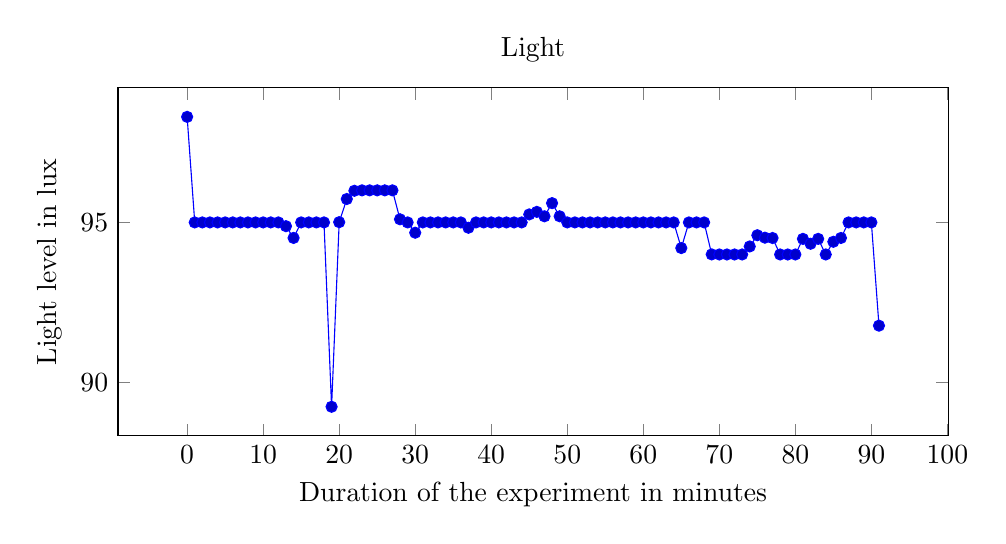
\begin{tikzpicture}
\begin{axis}[
	height=6cm,
	width=\textwidth,
	xlabel=Duration of the experiment in minutes,
	ylabel=Light level in lux,
	title=Light,
	unbounded coords=discard],
	
\addplot coordinates {
(0 , 98.2916666667)
(1 , 95.0)
(2 , 95.0)
(3 , 95.0)
(4 , 95.0)
(5 , 95.0)
(6 , 95.0)
(7 , 95.0)
(8 , 95.0)
(9 , 95.0)
(10 , 95.0)
(11 , 95.0)
(12 , 95.0)
(13 , 94.8825577778)
(14 , 94.5164273333)
(15 , 95.0)
(16 , 95.0)
(17 , 95.0)
(18 , 95.0)
(19 , 89.25)
(20 , 95.0078283333)
(21 , 95.7297625)
(22 , 95.986889)
(23 , 96.0)
(24 , 96.0)
(25 , 96.0)
(26 , 96.0)
(27 , 96.0)
(28 , 95.0976655)
(29 , 95.0)
(30 , 94.678594)
(31 , 95.0)
(32 , 95.0)
(33 , 95.0)
(34 , 95.0)
(35 , 95.0)
(36 , 95.0)
(37 , 94.8333333333)
(38 , 95.0)
(39 , 95.0)
(40 , 95.0)
(41 , 95.0)
(42 , 95.0)
(43 , 95.0)
(44 , 95.0)
(45 , 95.25)
(46 , 95.3285295)
(47 , 95.190542)
(48 , 95.601148)
(49 , 95.190604)
(50 , 95.0)
(51 , 95.0)
(52 , 95.0)
(53 , 95.0)
(54 , 95.0)
(55 , 95.0)
(56 , 95.0)
(57 , 95.0)
(58 , 95.0)
(59 , 95.0)
(60 , 95.0)
(61 , 95.0)
(62 , 95.0)
(63 , 95.0)
(64 , 95.0)
(65 , 94.2)
(66 , 95.0)
(67 , 95.0)
(68 , 95.0)
(69 , 94.0025184211)
(70 , 94.0)
(71 , 94.0)
(72 , 94.0)
(73 , 94.0)
(74 , 94.25)
(75 , 94.6)
(76 , 94.524485)
(77 , 94.5133925)
(78 , 94.0)
(79 , 94.0)
(80 , 94.0)
(81 , 94.48627)
(82 , 94.3333333333)
(83 , 94.486889)
(84 , 94.0)
(85 , 94.3959052)
(86 , 94.5150075)
(87 , 95.0)
(88 , 95.0)
(89 , 95.0)
(90 , 95.0)
(91 , 91.78003)
};

\end{axis}
\end{tikzpicture}
 	\vspace{5 mm}
\end{figure}

\newpage
\FloatBarrier
\newpage
\subsection{Noise Level}
\begin{figure}[ht]
	\centering
	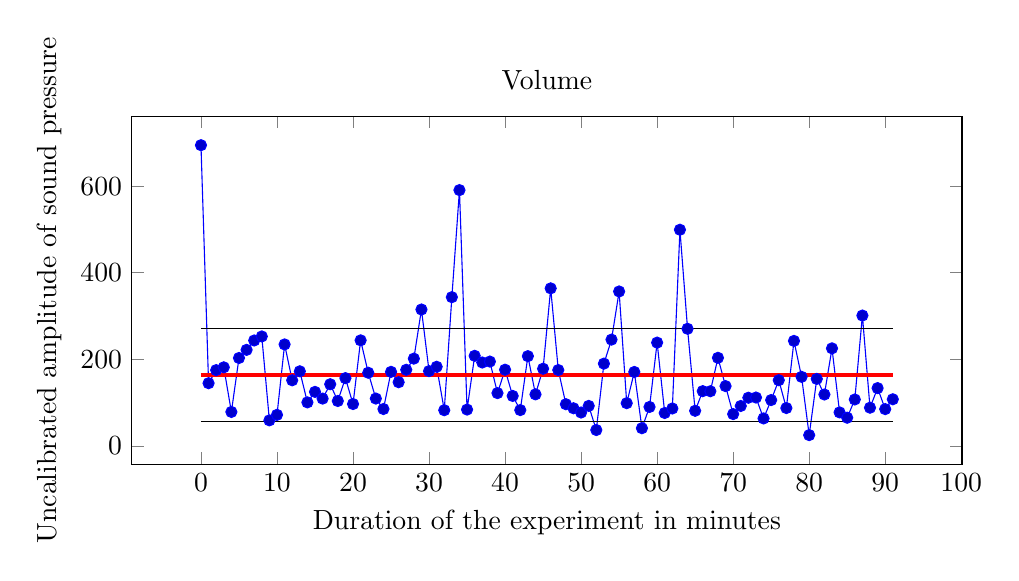
\begin{tikzpicture}
\begin{axis}[
	height=6cm,
	width=\textwidth,
	ylabel=Uncalibrated amplitude of sound pressure,
	xlabel=Duration of the experiment in minutes,
	title=Volume,
	unbounded coords=discard],

\addplot coordinates {
(0 , 694.416666667)
(1 , 145.086956522)
(2 , 175.285714286)
(3 , 181.7)
(4 , 78.75)
(5 , 203.25)
(6 , 222.0)
(7 , 243.666666667)
(8 , 253.0)
(9 , 59.3333333333)
(10 , 72.0)
(11 , 234.6)
(12 , 151.8)
(13 , 172.555555556)
(14 , 100.833333333)
(15 , 125.0)
(16 , 109.5)
(17 , 142.692307692)
(18 , 104.0)
(19 , 156.75)
(20 , 97.0)
(21 , 244.0)
(22 , 169.25)
(23 , 109.666666667)
(24 , 85.5)
(25 , 171.25)
(26 , 147.333333333)
(27 , 176.0)
(28 , 201.8)
(29 , 315.166666667)
(30 , 173.0)
(31 , 183.0)
(32 , 82.75)
(33 , 343.666666667)
(34 , 590.75)
(35 , 84.2)
(36 , 208.25)
(37 , 192.833333333)
(38 , 195.0)
(39 , 122.2)
(40 , 176.2)
(41 , 115.666666667)
(42 , 83.0)
(43 , 207.5)
(44 , 119.333333333)
(45 , 178.5)
(46 , 364.0)
(47 , 175.4)
(48 , 96.6)
(49 , 87.2)
(50 , 77.4)
(51 , 92.6666666667)
(52 , 37.0)
(53 , 190.25)
(54 , 245.666666667)
(55 , 356.8)
(56 , 99.0)
(57 , 171.0)
(58 , 41.2)
(59 , 90.25)
(60 , 238.75)
(61 , 76.3333333333)
(62 , 86.75)
(63 , 499.25)
(64 , 270.666666667)
(65 , 81.4)
(66 , 126.75)
(67 , 126.5)
(68 , 203.636363636)
(69 , 138.368421053)
(70 , 73.8)
(71 , 92.5)
(72 , 111.5)
(73 , 112.0)
(74 , 63.75)
(75 , 106.2)
(76 , 152.0)
(77 , 87.75)
(78 , 242.666666667)
(79 , 159.75)
(80 , 25.25)
(81 , 155.0)
(82 , 119.0)
(83 , 225.5)
(84 , 77.7)
(85 , 65.4)
(86 , 107.5)
(87 , 301.25)
(88 , 88.5)
(89 , 133.75)
(90 , 85.25)
(91 , 108.0)
};

\addplot[mark=none, red, very thick] coordinates {(0, 163.759695494) (91, 163.759695494)};

\addplot[mark=none, black] coordinates {(0, 56.1651969983) (91, 56.1651969983)};
\addplot[mark=none, black] coordinates {(0, 271.354193989) (91, 271.354193989)};

\end{axis}
\end{tikzpicture}
 	\vspace{5 mm}
\end{figure}

\FloatBarrier

\subsection{Location}
-6.250537, 53.3437789

Dublin, Ireland

\FloatBarrier